\documentclass[12pt,]{article}
\usepackage[utf8]{inputenc}
\usepackage{lmodern}
\usepackage{adjustbox}
\usepackage{graphicx}
\usepackage{grffile}
\usepackage{amssymb,amsmath}
\usepackage{ifxetex,ifluatex}
\usepackage{fixltx2e} % provides \textsubscript
\usepackage{longtable}
\usepackage{url,hyperref}
\hypersetup{unicode=true,
            pdfborder={0 0 0},
            breaklinks=true}
\urlstyle{same}  % don't use monospace font for urls

\usepackage{longtable,booktabs}
\IfFileExists{parskip.sty}{%
\usepackage{parskip}
}{% else
\setlength{\parindent}{0pt}
\setlength{\parskip}{6pt plus 2pt minus 1pt}
}
\setlength{\emergencystretch}{3em}  % prevent overfull lines
\providecommand{\tightlist}{%
  \setlength{\itemsep}{0pt}\setlength{\parskip}{0pt}}
\setcounter{secnumdepth}{0}
% Redefines (sub)paragraphs to behave more like sections
\ifx\paragraph\undefined\else
\let\oldparagraph\paragraph
\renewcommand{\paragraph}[1]{\oldparagraph{#1}\mbox{}}
\fi
\ifx\subparagraph\undefined\else
\let\oldsubparagraph\subparagraph
\renewcommand{\subparagraph}[1]{\oldsubparagraph{#1}\mbox{}}
\fi

\newcommand{\comment}[1]{\textbf{[[#1]]}}
\newcommand{\cfcmt}[1]{\comment{CFS: #1}}
\newcommand{\cfonly}[1]{\comment{CFS only: #1}}
\newcommand{\jdcmt}[1]{\comment{JD: #1}}
\newcommand{\mlcmt}[1]{\comment{MLi: #1}}


\bibliographystyle{plain}

\date{}

\begin{document}

\subsection{Manuscript}\label{manuscript}

\subsubsection{Title}\label{title}

Female Genital Cutting Is a Social Coordination Norm in Kenya, Mali, Nigeria and Sierra Leon
\cfcmt{This title is a response to Efferson’s title}

\subsubsection{Authors}\label{authors}

Chyun-Fung Shi (corresponding author), Department of Biology, McMaster
University. Michael Li, Department of Biology, McMaster University.
Jonathan Dushoff, Department of Biology, McMaster
University.

\subsection{journals}\label{journals}
possible consideration:  The Lancet Global Health, Science, BMJ, Bulletin of WHO

\subsection{Abstract}\label{abstract}

\subsubsection{Context}\label{context}

\subsubsection{}\label{objective}

\subsubsection{Methods}\label{Methods}

\subsubsection{Main Outcome Measures}\label{main-outcome-measures}

\subsubsection{Results}\label{results}

\subsubsection{Conclusions}\label{conclusions}

\subsubsection{Funding}\label{funding}

\subsubsection{Keywords}\label{keywords}

female genital cutting/mutilation, multilevel model, social norms, gender, DHS

\subsection{Introduction}\label{introduction}

It is estimated, based on a UNICEF global database including Demographic and Health Surveys (DHS), Multiple Indicator Cluster Surveys (MICS),  and other nationally representative surveys between 2004 to 2015, that more than 200 million women and girls have undergone female genital cutting (FGC), mostly in Africa and the Middle East and 44 millions of them are girls below age 15 \cite{UNIC16}.  Current progress in reducing FGC is insufficient to keep up with the population growth, and girls and women undergoing FGC will rise significantly over the next decade \cfonly{double check}) if the trends continue \cite{KhosBane17, UNIC16} (also see \url{http://www.who.int/mediacentre/factsheets/fs241/en/} updated Sep, 18).  FGC is also known as female genital mutilation and female circumcision; we use cutting instead because it implies a degree of self-awareness and is considered less judgmental \cite{KhahBark09, JohnEsse10, Meye00, PariSaru18, Shel01}  \cfonly{To rethink differences between FGC and FGM.  The types of FGC vary from just a knick to a sever sewing of the genital area.  Using FGC(cutting) seems to ignore the damage to the girls and human rights, but FGM(utilization) seem harsh and biased against local cultures.  FGC(cirumcision) may be the best for current situation globally.)

The commonly shared position for FGC is more about eradication than intervention \cite{KhosBane17, Mack96, Toub94, UNIC16, WHO97}, as the United Nations has declared that FGC as violates human rights, and promoted the abandonment of the practice  \cite{WHO97, WHO08} \cfonly{add and update}.  The progress is hindered due to the complicated history of the very practice \cite{Cami16}. The meanings of FGC are competitively defined by various groups from local religious community to international governmental institutes, by linking the practice to cultural and religious identity in one end and to public health and human rights on the other \cite{AhmeKare18, BergDeni13a, Boyl02, KhosBane17, KimaShell18, SchuLien13, WHO12}.

Social norm is a fundamental approach in comprehending and intervening FGC practice \cite{DuncWand11, EffeVogt15, Hayf05, Mack96, Mack00, Youn02} while other perspectives (e.g., human rights and feminist theory \cite{Dell04, FrieMahm13,KhosBane17, Lewi95, Lewi09, Meye00, Morr08, Njam04, UNIC16, YirgKass12, Youn02} entails reasons of negotiating and abolishing the practices.  Convention theory posits FGC an important norm to control marriage fidelity and social prestige; this perspective views FGC as a social behaviour resulting from group practice, and it takes a ``critical mass" to initiate a change \cite{Mack00, MackLeJe08}.  FGC was also viewed as a social capital for inclusion and exclusion within women’s social groups \cite{Shel-Wand11}.  When the norms within the communities are strong, individuals tend to self-enforce community norms \cite{Ajze02, Hayf05, KandNwak09, Mack96, Mack06, MackLeJe08, ThomMadd92} and the bond within women's social networks could be intergenerational, interdependent and interconnected across generations and genders was proposed intervention of FGC  \cite{Mack00, DuncWand11, ShelWand11}. \cfonly{add \cite{Bicc15}}

\cfonly{add \cite{AlcaGonz13, BellNova15, PashPonn16, Rima08, ShelWand11, more} and other norm studies of why mother cut daughters etc}

Although convention theory was well deliberated and applied and showed a larger effect on FGC practices than the others (e.g, \cite{BoylMcMo02, BoylCorl10, FreyJohn07, FrieMahm13, Hayf05, KandMwek09, Mack96, Mack06, ReigGonz14, YirgKass12}),  it was not without challenges \cite{EffeVogt15} and multiple theoretical frameworks were called to be incorporated to grasp a full explanation of the persistence and decline of FGC due to the heterogeneity of the population \cite{EffeVogt15, ModrLiu13}.  

% prevalence of FGC in those 4 nations.

\subsection{Research Questions}\label{research-questions}

Identifying benefits of FGC practice is crucial to promote sustainable change \cite{EffeVogt15}.  This study takes both the dynamics of beliefs of FGC benefits and of FGC practices into account at both a population and a community level to understand associations of FGC values and intention of carrying out the practices l \cite{BoylCorl010, Drol11,Hayf05, HayfTrin11, Grue05, Hodg11,KandNwak09, OdukAfol17} (to confirm).  We developed three models in this study.  The main one is the “daughter” model, which analyzed associations of beliefs of FGC benefits (see the list of FGC benefits at table xx) and intention to cut daughters in the hope that if patterns of social norms (i.e., aggregation of values of FGC benefits) associating behavioral intention can be detected.  Additionally, we also decompose the model into two “structural” models:  “persistence” model to study women’s beliefs of FGC benefits and FGC continuance; and “future” model to examine the association of beliefs of FGC benefits, FGC persistence and intention of cutting daughters to understand how such positions change the main model.

\subsection{Methods}\label{methods}

\subsubsection{Data and Samples}\label{data-and-samples}

We analyzed the Demographic and Health Surveys (DHS) by USAID.  Countries with the following criteria were selected:  high FGC prevalence \cite{UNIC16}, DHS surveys with modules of FGC benefits, and index of gender awareness; and that resulted in four nations:  Kenya 2008/9, Mali 2006, Nigeria 2008 and Sierra Leone 2008.  We did not analyze the newest dataset due to the lack of FGC benefits modules before this study finished for publication (checked in 1/09/19).

Only women with daughters to be considered for FGC were included in 
 main model (the daughter model) and the future-daughter model, while the future model included all the women in the samples; that resulted in xxx, xxx and xxx (or three more if sample sizes in individual models are different from the full models) respectively.
\cfcmt{FGC module at \url{https://dhsprogram.com/pubs/pdf/DHSQMP/DHS5_Module_Female_Genital_Cutting.pdf}}

\subsubsection{Measurements and Concepts}\label{measurements-and-concepts}
\cfonly{\cite{Rima08}}*

Our main interest in this project is to study how norms associate with behavioural intention.  We focus on how women will likely cut their daughters or not based on their current intention and that provide a more convincing result on how FGC norms affect FGC practice than using than what had already happened (e.g. women’s own FGC status).  Therefore, our main response variables were woman's behavioural intention to cut their daughters in the daughter model and the mixed (daughter-future) model, and woman's attitude on whether FGC should be continued in the FGC persistence model.  The predictors were selected based on literature and three main theories which have developed to account for the practice of FGC (i.e., convention theory, feminist theory and modernization theory) \cite{Fay05, BellNova15}.  The main predictors were woman's FGC status, beliefs of FGC benefits and attitudes of gender equality.  Beliefs of FGC benefits was estimated based on a list of questionnaires (see supp) and quantified using PCA in order to identify which benefit was mostly recognized in connection norm.  Other socio demographic variables were also included:  age, education, religion (see the list of religion recode at table xx in appendix; with a footnote on how we recoded it), marital status, work status, media and residence (urban vs. rural) in addition to country.  The followings were treated as random variables:  cluster ID (villages) and ethnicity (see the list of ethnicity recode at table xx in appendix; with a footnote on how we recoded it).

In order to address the significance of community impact on the practice of FGC, education, wealth, media use, FGC beliefs, gender awareness and FGC prevalence were also tested at the community level \cfcmt{on a cluster level, not national, right?} in response to the degrees of modernization, conventional values and gender awareness within- and among-community (see \cite{Achi14, BoylMcMo02, Hayf05, KandNwak09, ModrLiu13, Moor13, OdukAfol17, Youn02}).}).  Cluster  was used as a proxy to represent a community level of impact \cite{AligRen06, Hayf05, Krav02}

\jdcmt{Ideally, we would make ethnicity a random effect, but we are back to the Gilmour problem I guess.} \cfcmt{Ethnicity is an important factor (see Hayf05), more so than religion, associating with FGC status, and I don't think it shall be coded as a random factor.  But as J said, it is too hard! } %``explicitly including ethnicity is a means of assessing another dimension of the collective aspect of circumcision behavior. `` \cite{Hayf05}
\cfcmt{Bayesian model \cite{KandNwak09} ``Conversely, one cannot assume that the clusters selected in each district are fully representative of the states in which they are located because surveys only attempted to generate a fully representative sample at the regional level. Consequently, the spatial analysis will be affected by some random fluctuations.  Some of this random variation can be reduced through structured spatial effects because it includes neighboring observations in the analysis. However, it should be pointed out that such a spatial analysis should preferably be applied to census data, where the precision of the spatial analysis would be much higher." (p. 788)}
\cfcmt{Regarding FGC benefits modules, there were 9 questions.  Keya had all the 9, Mali and SL 7 (missing promiscuity and STD), NG 8, missing STD).  Should we drop STD since 3 out of 4 missed this variable?}

\subsubsection{Statistical Model}\label{statistical-model}

We used cumulative link mixed models (CLMMs) in the statistics package R \cite{Rstats,Rpackage_ordinal} to analyze the models.  The CLMM framework allows us to model a binary or ordinal response variable (i.e., intention of cutting daughters and whether to continue FGC practice), while treating clusters and ethnicity as random effects.  
We subtracted respondent (-1) from the cluster when testing the community effect \cfjd{Please rewrite this. Also, do we need to mention how we treat cluster with only one sample (if that happens).}

\cfcmt{Our response ARE categorical not binary; AND still need to explain why ethnicity is a random effect. AND media use was supposed to be incorporated as a random factor at the country level, based on the assumption that media content likely varied among countries.}

\cfcmt{reference: Methods and the first paragraph of Discussion\cite{Chia14}}


\subsubsection{Scripts}\label{scripts}

Codes are be available upon request. 


\subsection{Results}\label{results-1}

Baseline socio-demographic and sample characteristics are shown in xxx.  The prevalence of FGC are \%, \%, \% and \% in Kenya, Mali, Nigeria and Sierra Leon accordingly, and \%, \%, \% and \%  of the samples thought FGC should continue as well.  

The results of the three models are at ____.  The findings showed that all the three responses were clearly associated with the following predictors:  women’s fgc status, beliefs of fgc benefits and FGC prevalence in a community; so as the following factors:  country, media, education, age and religion and the community levels of media, education.  We did not find clear association of the community level of beliefs of fgc benefits and the three responses.


\cfcmt{main predictors:  beliefs of FGC benefits, woman's FGC status and attitudes of gender equality}

Tables and figures to be included:
- table of basic sociodemographic results
- 3 figures of the results of the 3 models
- a figure of women’s FGC prevalence vs. their intention of cutting daughters vs. attitudes towards FGC continuity.  (ref to \url{https://www.ncbi.nlm.nih.gov/pmc/articles/PMC3302551/}, Fig 1)
% figure:  plots of FGC benefits (This figure will be important. It tells us what women thinks about why FGC).
% figure: to put the first PCA of FGC believes of the 4 nations at the community level and maybe in one figure
% a chart like figure 8-8D \cite{UNIC13}



\subsection{Discussion}\label{Discussion}

--Main interpretation --

Our findings suggest that a daughter’s likely future of being cut or not is overdetermined by her community’s overall likelihood of mothers’ intention of cutting their daughters, fgc prevalence, among others.  Our findings show that omen’s decision on cutting their daughters was clearly related to their own FGC status, personal beliefs of FGC benefits and theFGC prevalent in their community \cf{link}; yet group beliefs of FGC benefits in their community did not play a clear role in determining whether a daughter would be cut.  The similar results also applied to women’s view of whether FGC should be continued \cf{link}.  \cfjd{How to use the future-mother producing daughter model?}.  Our findings suggest that FGC practice is a social norm in respect of how an individual behavioral intention on FGC is in line with how their community implement this ritual; the social norm is based on what an agent perceives what their community members think and that perception can be based on the members’ behavioural outcome (i.e., whether others had FGC) or communication about the ritual practice \cite{} .
 


— Norm —

- conventional \cite{FreyJohn07, Hayf05, KandShel19, Mack96, ShelWand11} vs. 
- “attitude is the strongest predictor of mothers' intentions to allow their daughters to undergo FGM, followed by subjective norms." \cite{PashPonn16}. “alternative convention/peer convention\cite{ShelWand11}
 \cite{ShelWand11} proposed that reasons for fgc practice go beyond the belief that it is advantageous for marriage prospects. FGC allows women to gain social capitals and access to networks.  Their findings also suggested that the main deterent to marriages was not men's refusal of non-fgc women, but hostility and discrimination from fgc women to non fgc women}.  \cfonly{Mackie's social convention theory was supported in \cite{ShelWand11}.  In \cite{MackLeJe08}, the authors saw marriageability was only one reason for FGC and proposed multiple factors in influencing women’s decision of cutting their daughters.

\cite{PashPonn16}: Attitude was the strongest predictor of mothers' intentions for their daughters' FGC status, followed by subjective norms 


- community level of effects -
\cite{ChegAske04}(community -based approach), \cite{BrowBeec13, Hayf05, KandShel19, PatrSing15, ShelWand11}
\cite{BellNova15}: "We find that much of the variation in a woman's support for FGC can be attributed to individual- and household-level factors rather than to village-level factors or to factors beyond the village level."
- tipping point/threshold -
\cfcmt{empirical norm:  enough others follow the norm-  community level of FGC \cite{Bicc10} normative norm:  enough others think we need to follow the norm -  FGC beliefs, decision on daughter's FGC status (already and future), \cite{Bicc10}}

What does it mean that group level of daughter future as the biggest predictor compared to individual benefit and group fgc (prevalence)?  Does it mean that fgc norm works implicitly and it might not be something behaviour women really agree with?  Is it a social norm supported by social sanction (i.e., cutting daughter) for what reason? (see \cite{MackLeJe08} (p.28 which mentioned Bicchieri06)

- Beliefs of FGC benefits -
Our PCA results show that women’s beliefs of what benefits FGC brings is not clearly identified (see figure pca) and marriageability was not a clear one (to compare with \cite{Mack?,}.  On interpretation is that marriageability is no longer a strong belief in community where FGC is still common and new norms are insinuated around \cite{EffeVogt15, MackLeJe08, ShelWand11, networking, part of social groups Duncan-Shell?}

— secondary analysis/socio demograhpic —

- modernization (cite{BoylMcMo02, Youn02}, education and wealth as index of modernization), vs. gender \cite{Dell04, FrieMahm13, Lewi04, Meye00, Njam04, YirgKass12, Youn02}. 
 \cit{Hayf05}  Wealth:  Some research showed that household wealth has nonlinear correlation with women's FGC status predictor of daughter's FGC status
\cite{KandNwak09,VanMeek15} proposing various factors impacting FGC practices, such as women's education 

\cite{MashMatt09} (In Ethiopia):  Women who believed that FGM should continue were more likely to be aged 15-24years; rural residents; Muslim; married ; uneducated ; circumcised ; and to have had no exposure to mass media
\cite{DalaKalm18}(in 7 African countries): increasing media coverage and education, and reducing poverty are of importance for shifting adolescent girls' attitudes in favor of discontinuation of FGM.
\cite{Hayf05, PashPonn16} (more)
% education:  \cite{IliyAbub12, KarmKand11}
% religion:  \cite{HayfTrin11, KarmKand11}

— by nations and laws in those nations—

%Except for Mali, all the studied nations have enacted decrees or legislation related to FGC \cite{WHO13}

In Ethiopia, the majority of women who were aware of the negative reproductive health effects had not stopped the practice highlighted the possible fear of isolation and being alienated from the cultural system where FGC could be seen as a force of social cohesion \cite{YirgKass12}.  In Kenya, woman's decision on whether to cut their daughters' genitals were likely to relate to collective identity within ethnic groups against broader social changes \cite{Achi14, Hayf05}; similarly findings observed in Nigeria \cite{FreyJohn07, KandMwek09}.


---- Kenya: legal background:  Kenya \cite{GKEN01}; \cite{UNIC13}; 
 vs. \cite{Chia14, Hayf05}, and [\url{http://kenya.usaid.gov/programs/women/182 PEPFAR/kenya}]
---- Mali: ``The occurrence of FGM/C is also concentrated in certain West African countries where prevalence rates range from 72–96 percent: Burkina Faso, the Gambia, Guinea, and Mali. The populations of these countries share certain social and historical ties, which suggests that a strategy to eliminate FGM/C in one of these countries might be successful in others. FGM/C is practiced as part of the initiation into a secret society in Liberia and Sierra Leone. We should expect that the repercussions for mothers there who do not send their daughters to be initiated would be different than for mothers in nearby Mali or Guinea \cite{YodaWang13}

---- Nigeria: ``Modernization (education and high socioeconomic status) had minimal impact on the likelihood of FGM, but education plays an important role in the mother's decision not to circumcise her daughter. It follows from these findings that community factors have a large effect on FGM, with individual factors having little effect on the distribution of FGM" \cite{KandNwak09}

---- Sierra Leone: 
\cite{Sagn14}  

— Suggestions —
- empowering community, engaging community leaders and other strategies \citeBergDeni13b}
- MC vs. FGC.  Considering the acceptance of Alternative rights of passage \cite{GaluKama15} without criminalize the practice. (I'm not sure if I'm comfortable with this position, but it is an alternative.) vs. focused on empowerment, and campaigns to recruit change agents from within communities (to eradicate FGC) \cite{ShelHern13, Will18}
- modelling by plotting empirical data to study threshold/tipping point.
- redesign questions of fgc benefits in DHS
- inviting faced women migrated to western society to participate in fgc intervention campaign.  For example,  attitude change: "migrating to and living in Sweden facilitates a transition in attitudes regarding FGC" \cite{WahlJohn17}

— Limitation —
- No FGC types relating to our response varialbes


\subsection{Conclusion}\label{Conclusion}

==================================
\cite{Drot11, Grue05, JoneEhir04} (both on cultural perspective, and maybe norm), 

--- attitudes vs. norm (beliefs) vs. (behavioural) intention (intended behaviors, planned behavior, controlled behavior) \cite{Ajze02, ThomMadd92}
\cite{TerrHogg96}:  subjective norm on attitude and planned behavior.  There were three main predictors of intention:  attitude, norm and perceived behavioroal control.

\cite (The social construction of reality: a treatise in the sociology of knowledge Anchor Books, New York, NY (1966))


OVERALL:
\cite{UNIC13}:  “Many girls who are cut are daughters of women who oppose the practice” 


% The findig “suggests that even with a sharp decrease in FGC prevalence, the bulk of FGC persistence would still come from household-level factors. This is in contrast to the tipping point and informational cascade models … , wherein the decision to abandon a social norm such as FGC should be entirely individual in places where the practice is highly pervasive.”  they found that “that much of the variation in a woman's support for FGC can be attributed to individual- and household-level factors rather than to village-level factors or to factors beyond the village level”  \cite{BellNova15}; and to compare our results to \cite{BellNova15} because they agnostic about the three theories.

\comment{cf: how to cite \cite{AkhmWord13,EffeVogt15} and compare these two?}
% There are "discrepancies between attitudes and practices, especially significant under an analysis by sex as, despite manifesting less support, the percentage of female HCPs declaring to have performed medicalization is almost twice the males' average. These findings suggest that female HCPs could be facing higher demand to medicalize the practice, and that, even when brought to the medical setting, FGM/C is regarded as a women's issue to be performed by women to women." \cite{KaplSing16}

% "autonomy within culture" is socially situated and entails neither endorsement of FGC nor resignation to its persistence." \cite{Meye00}:  How can we apply this feminism perspective to our findings? (Since we did not categorize types of fgc in our study, we can't know if women of autonomy prefer to have a "nick" on their daughter to preserve cultural identity or abandon fgc completely.

% \cite{WahlJohn17} showed that change does occur in newly immigrants once they were relocated to a new society where FGC was defied; how does this compared to \cite{EffeVogt15}'s heterogeneous model?


% little support for seeing FGC a prerequisite for marriage or related to marrying well, but peer pressure was an important factor on FGC decision (i.e., peer convention instead of marriage convention.) \cite{DuncWand11}
% when influences from within the communities are strong, individuals tend to self-enforce norms of what the community expect from their behaviours \cite{Hayf05, KandNwak09, Mack96, Mack06, MackLeJe08}. (from the introduction.  try to compare our result with theirs).
% mother-daughter: \cite{PashPonn16}



% Overall:


%Because of the social aspects associated with FGC, including gender norms and power relations, it is fundamentally important that intervention of FGC practice adopts a holistic approach to focus both on individual and the wider social dynamics \cite{BrowBeec13}. 
 \cite{Shel-Wand11}:  supporting Mackie's convetion theory ``expections regarding fgc are interdependent...."

% suggestions:  to invite elder woman to participate in reducing FGC \cite{ShelMore18}

% contagious diffusion \cite{Mack96}

% ``FGC facilitates the accumulation of social capital by younger women and of power and prestige by elder women. Based on this new evidence and reinterpretation of social convention theory, we suggest that interventions aimed at eliminating FGC should target women's social networks, which are intergenerational, and include both men and women. Our findings support Mackie's assertion that expectations regarding FGC are interdependent; change must therefore be coordinated among interconnected members of social networks." \cite{ShelWand11}

FGC is still in practice or a preference among women after migrated to a western environment from their original communities where FGC was a common practice, in the hope (wording?) of preserving their ethnic and gender identity despite its conflict against the  norms and laws of the newly settled society \cite{}; however, a baseline study in Sweden showed that a majority of female immigrants, including those newly arrived, opposed all forms of FGC with increased opposition over time after migration, and suggested that an attitude change had occurred \cite{WahlJohn17}; that suggested a likely influence of convention theory.


% Spatial Bayesian model \cite{KandNwak09}
% idea of purity of women reflects on the status and honor of their families \cite{Ortn87}.  Female purity is oriented to an ideal and unattainable higher class. \cite{Ortn87}
% a possibility of a multicultural egalitarian society \cite{Wade11}
% success in community education program to abandon FGC \cite{DiopAske09}
%\cfcmt{convention theory mainly work on norms or also on behaviour change?  There seems a gap between norm and behaviour in FGC, can diffusion theory brigade the gap?  As suggested, community-based education program has fallen shot tin changing FGC behaviours \cite{Shel08}}
% "I do not deny that individuals have evolved the capability to learn and apply social norms even to situations that are completely new, but there is much evidence that we are conditional followers of norms. In fact, as the experiments reported in Bicchieri and Xiao (2009) and Bicchieri and Chavez (2010) show, manipulating information produces major changes in behavior, and the existence of a social norm is no guarantee that it will be followed. The real challenge we face is to explain how normative expectations emerge or, in other words, how the beliefs that support social norms take shape." \cite{Bicc10}.


“we find that some older women express an openness to reassessing norms and practices as they seek solutions to maintaining the physical well-being, moral integrity and cultural identity of girls in their families. Moreover, given the authority of older women over younger women, they also have power to negotiate change.\cite{ShelMore18}

% "granted, recognized, and implemented by the state must not de-emphasize or delegitimize approaches recognizing the cultural significance of FGC and the potentially multiple and cascading social effects of ending the practice." \cite{(Shel08}, p. 229)


% A society may discontinue FGC practice or maintain the practice in a different form (e.g., a less harmful type of FGC) (that is cultural change in Wade's concept \cite{Wade11})

%  "Residual spatial effects of FGM have enabled us to see the inherent spatial patterns of the prevalence of FGM because the variability or noise has been removed. A more precise spatial pattern of the prevalence of FGM emerged with the estimated residual state effects compared with the crude prevalence without the control of geographic location effects." \cite{KandNwak09, p. 791}


% From modifying the practice to discarding it through a process of conversations and understanding  \cite{Mutu02, Shel08}
% findings in \cite{BoylMcMo02}
%* "These finding are particularly informative because most modernization analyses only consider attitude change. The most plausible interpretation is that attitudes change before behavior, and that our analysis captured women in the midst of change." (p. 22)
%"The greater probability of favoring FGC in Egypt was statistically significant compared to all other countries;" (p.22) (This finding is against modern theory/development theory).
%"Our findings suggest that regional development influences attitudes and behavior, but national resistance to international norms can outweigh the influence of regional development." (p.23)
%* "We hypothesized that those carriers of the scripts of the international system – education, mass media and working in the paid economy – would affect women's attitudes and behavior with respect to FGC. These hypotheses were confirmed" (p. 23) "Older women were less likely to favor the continuation of circumcision, although each year of age increased the probability that a woman had or planned to circumcise her daughters by 6 percent. Older women may have cut their daughters before there was international pressure opposing the practice. The reverse effect for attitudes is consistent with prior findings (see Williams and Sobieszczyk, 1997). It may be an artifact of the survey technique. Older women who oppose FGC may feel freer to say so than younger women because older women are accorded considerable independence in Muslim societies (see, for example, Geiger, 1997).20" (p.24)

% "This study suggests that the adoption of a `modern' lifestyle is not an inevitable result of acquiring the tools that give a person mastery over nature. Rather, the transmission of particular ideologies through global institutionalized arrangements appears to be the critical factor in abandoning practices like FGC." \cite{(BoylMcMo02}, p. 26)  What does this mean???


% National and cultural boundaries are not coextensive, when religious and community-based norms are considered \cite{BoylCorl10} (similar cultural approach \cite{SchuLien13}

% The legitimacy of international laws banning the practice of FGC"rests on its ability to demonstrate that global and local cultures are highly interpenetrated—that global culture absorbs a full range of local values." \cite{(BoylCorl10}, p 209)

% Festinger's cognitive dissonance theory:  a condition of conflict results from inconsistence between one's attitudes and one's beliefs.

% "In 1997, the Ministry for the Promotion of Women in Mali created a National Committee Against Violence Towards Women that links all the international organizations active in preventing FGC in Mali" "In 2001, the Kenya legislature adopted a law banning FGC." "the founding father of the country (Kenyatta, 1962) explicitly linked FGC to nationalist pride."

%"This review demonstrates the strong social pressure to which women are subjected as regards the practice of female genital mutilation. However, many other factors can contribute to eroding beliefs and arguments in favour of this practice, such as the globalization, culture and social environment of countries in the West." \cite{ReigGonz14}



systematic review of effectiveness of fgc factors associating the practice \cite{WaigDoos18}

Gender/feminist perspective:  \cite{Meye00} Meyers questions the idea of social norm and autonomy "It seems to me that we would need far more consensus than we presently have (or are likely to get) about human nature and social justice before we could conclude that women who opt for compliance with female genital cutting norms never do so autonomously.  We would have to be persuaded, in other words, that all women's interests are such that this decision could not accord with any woman's authentic values and desires under any circumstances." 

Egypt:  "Literate, better educated and employed women are more likely to oppose FGM" \cite{VanMeek15}
Sinegal: \cite{KandComb15}
West Africa:  \cite{SipsChen12} (law and current practices)
Theory:  

% convention or modernization theory?`` campaigns against FGC using educational, health, legal, and human rights–based approaches are at times ineffective and counterproductive when they frame the practice as a ``tradition" rooted in a ``primitive" and unchanging culture. We suggest that development interventions that do not address local contexts of FGC, including the complex politics and history of interventions designed to eradicate it, can in fact reify and reinscribe the practice as central to Maasai cultural identity." \cite{WintKoom09}

% \cite{Koom14}: `` practices of female excision are so diverse that they may defy generalizable remedies"  ``Rather than relying on common campaign models, transferable advocacy tools, or `best practices,' scholars and anti-FGM activists must rethink female excision in terms of its diverse contextual meanings and its dynamic global politics."  Instead of straightforward campaigns against traditional culture, "culturalconstestaion" characterized by politicized negotiation and, at times, resistance, was proposed. \cite{Koom14}.

A multicultural egalitarian approach respecting both cultural identity and basic legal human rights was addressed \cite{BoylCarb10, Wade11}.  


% "Tradition, cleanliness, and virginity were the most common motives empowering the continuation of FGM/C , followed by men's wish, esthetic factors, marriage, and religion factors.... A variety of socio-cultural myths, religious misbelievers, and hygienic and esthetic concerns were behind the FGM/C. Overall, a large proportion of the participants supported the continuation of FGM/C in spite of adverse effect and sexual dysfunction associated with FGM/C." \cite{MohaHass14}

% read \cite{MohaHass14, MuteMill16, PashPonn16, VaroFras14}

"support HCPs in the integration of FGM/C preventive interventions within the public health system, to address arguments favoring medicalization, and to use data to design appropriate strategies." \cite{KaplRiba16}

% norm/attitude vs. behaviour:  attitudes towards fgc did not have a positive correlation with their behaviour:  ``within each country women from more developed regions, women who worked outside the home, and educated women were less likely to favor genital cutting and less likely to have their daughters cut. Living in an urban area decreased the likelihood of favoring genital cutting, but it had no effect on behavior. `` \cite{BoylMcMo02}

%\cfcmt{Bicchieri's norm theory \cite{Bicc06}:
behaviour:  What the responder do 
personal normative behaviour:  What the responder believes she should do
empirical expectation:  What the responder believes others do
normative expectation: What the responder believes others think she should do


\cite{UNFPA14, UNIC16}

% cultural sensitivity:  It suggests that "legislative efforts to protect women's health may remain ineffective with
out structured efforts between health systems, governments or legal institutions and the cultural society." \cite{Iyio12} and 
% through laws \cite{AloGbad11}


% Education programs aimed to empower women through a broad range of educational and health-promoting activities by improvements in knowledge about and critical attitudes toward FGC had impact on behaviors and attitudes. \cite{DiopAske09}.  Legal measures must combine with social measures to effectively eradicate FGC and communities practising FGC must be involved in the planning and implementation of  intervention of FGC elimination \cite{AkoAwke09}

% \cite{BrowBeec13}:  their questions of the 4 current approaches (sexuality, human rights, etc) and their suggestions

% attitudes change may be followed by behaviour change, but more slowly \cite{BoylMcMo02}

%\cite{JohaDiop13}:  Some of the most common approaches (1) health risk approaches, (2) conversion of excisers, (3) training of health professionals as change agents, (4) alternative rituals, (5) community-led approaches, (6) public statements, and (7) legal measures.

% Did our findings see something like group/community identity, womanhood \cite{Koom14}?
% \cite{Koom14}: `` an Aang Serian activist who had addressed a village meeting saying, `The world is changing and the Maasai must change with it or risk dying out.' They argued that these appeals to cultural survival were much more persuasive and meaningful to them than the `foreign' language of rights."

Analyzing why MC is a much accepted behaviour might help us to re-think the meanings of FGC (see \cite{DarbSvob07}) and, if, to certain extent, to accept a form of FGC practice (e.g, a "nick" \cite{Wade11}).

% (Against common belief of a critical mass, an empirical model showed that FGC was not driven by a social norm based on coordination and there was no signal critical threshold for the practice because of various heterogeneity of the population \cite{EffeVogt15} \cfcmt{Can heterogeneity explain the differences of beliefs in FGC benefits at individual level vs. at a community level?}


% \cfcmt{TOSTAN uses a strategy based on convention theory's critical mass to eradicate FGC (see (Wils13}}
 * Festinger (1950?):  Social pressure in informal groups

% a chart to show changes of FGC prevalence from 2000 to the current surveys (Kenya 98, 03; Nigeria 99, 03; Mali 01, 06?  (see \cite{BoylCorl10}, table 1)

\cite{EffeVoge15}:  Each family may have its own threshold of fgc. I think fgc norm has shifted from marraige advantage of social capital of social networking as proposed by Shell-Duncon and her colleagues \cite{ShelWand11}.  To elaborate the shifted values of fgc, what it imply and how to apply the change to policy.
\cite{CentBeck18}:  social convention and tipping point

% suggestions: https://www.theguardian.com/global-development/2018/feb/06/battling-fgm-uganda-kenya-zero-tolerance-female-genital-mutilation "Thomas Lotongar, assistant chief in Konya Division in Kenya, says more rescue centres are needed, and schools must act as sanctuaries for girls to avoid FGM.  ``We need to find more alternatives and livelihood projects like tailoring[or] salon work to empower our girls who run away from the practice to the rescue centres.""



Suggestions: pricking (type IV\cite{WHO08})\cite{WahlJohn17a, WahlJohn17b} and medical FGC \cite{KimaShell18} vs. no-tolerance, fgc vs. mc \cite{WahlEsse18}?  We suggest to position ourselves in a context where male circumcision (MC) is practices and accepted; to consider the differences of a prick of FGC and MC; to comprehend the outcomes of abolishing FGC vs. changing FGC practices.
\cite{WahlEsse18}:  from sameness to differences, a global multicultural approach especially during the international migration across the globe.


\subsection{Conclusion}\label{Conclusion}

%"targeting women and girls is a sound investment, but outcomes are dependent on integrated approaches and the protective umbrella of policy and legislative actions" to change gender norms among women and girls \cite{KeleFran}. 
Reasons of FGC is not universal and different from community to community and from society to society; campaigns of reducing and preventing FGC need to incorporate with local history and believes.
% call for eduction in communication of FGC:  \cite{Koom14, Meye00}}

Eradication of FGC is more controversial than expected.  FGC practice and its nature tended to be morally embraced, and deeply internalized \cite{SchuLien13}.  Decisions on undergoing FGC was often a result of a collective practice than an individual choice \cite{Dell04, Hayf06, FreyJoh07, KandMwek09, Mack96, Mack06, ShelHern06, ShelWand11, YirgKass12}. Public denouncements and anti-FGC laws could push FGC into private practices \cite{GaluKama15, VanCoen17}.  Given the regional FGC prevalence, variations among countries and the social context of FGC practices (e.g., see Burkina Faso \cite{KarmKand11} vs. Nigeria \cite{KandNwak09}), a ``one size fits all" strategy for the abandonment of FGMC would not be effective \cite{JohaDiop13, YodeWang13}.



====================================
\subsection{Funding}\label{Funding}

CF was funded by a grant from the James S. McDonnell foundation. JD holds a New Investigator award from the Canadian Institutes of Health Research.

\subsection{Conflicts of interest}\label{Conflicts-of-Interest}

The James S. McDonnell foundation and the Canadian Institutes of Health Research had no role in study design; collection, analysis, and interpretation of data; the writing of the manuscript; or in the decision to submit the manuscript for publication.  The views expressed herein do not necessarily represent the views of the founding bodies.

\subsection{Authors' contributions}\label{Authors'-contributions}

\subsubsection{Disclaimer}\label{disclaimer}

The findings and conclusions of this article are those of the authors
and do not necessarily represent the views of the funding agency.

\subsubsection{Acknowledgement}\label{Acknowledgement}
Ben Bolker,  Marta Wayne

\subsubsection{Appendix}\label{appendix-1}

\FloatBarrier

\section{Figures}

\subsection{Daughter Plan}
\begin{center}
\begin{figure}[h!]
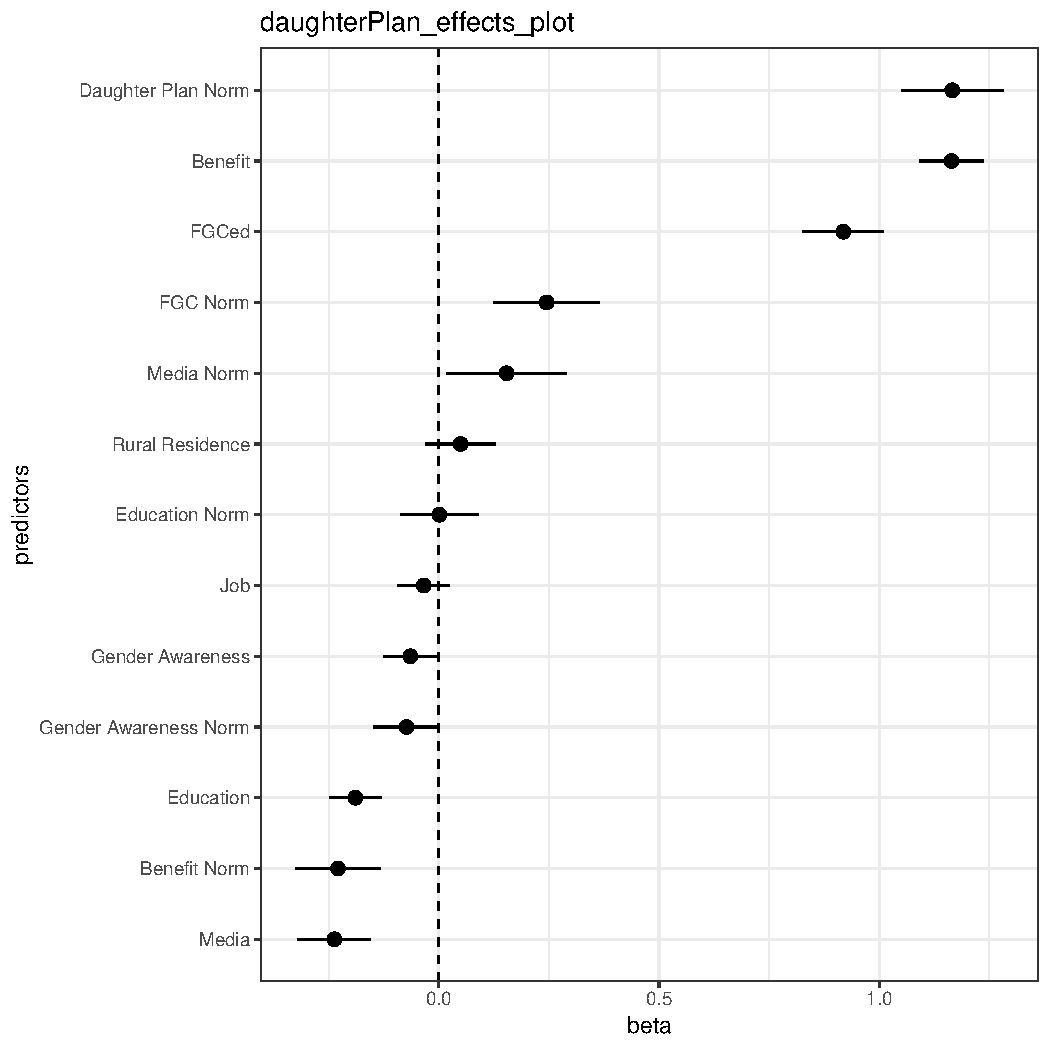
\includegraphics[scale=0.7]{./git_push/daughterPlan_effects_plot.Rout.pdf}
\end{figure}
\end{center}

\begin{center}
\begin{figure}[h!]
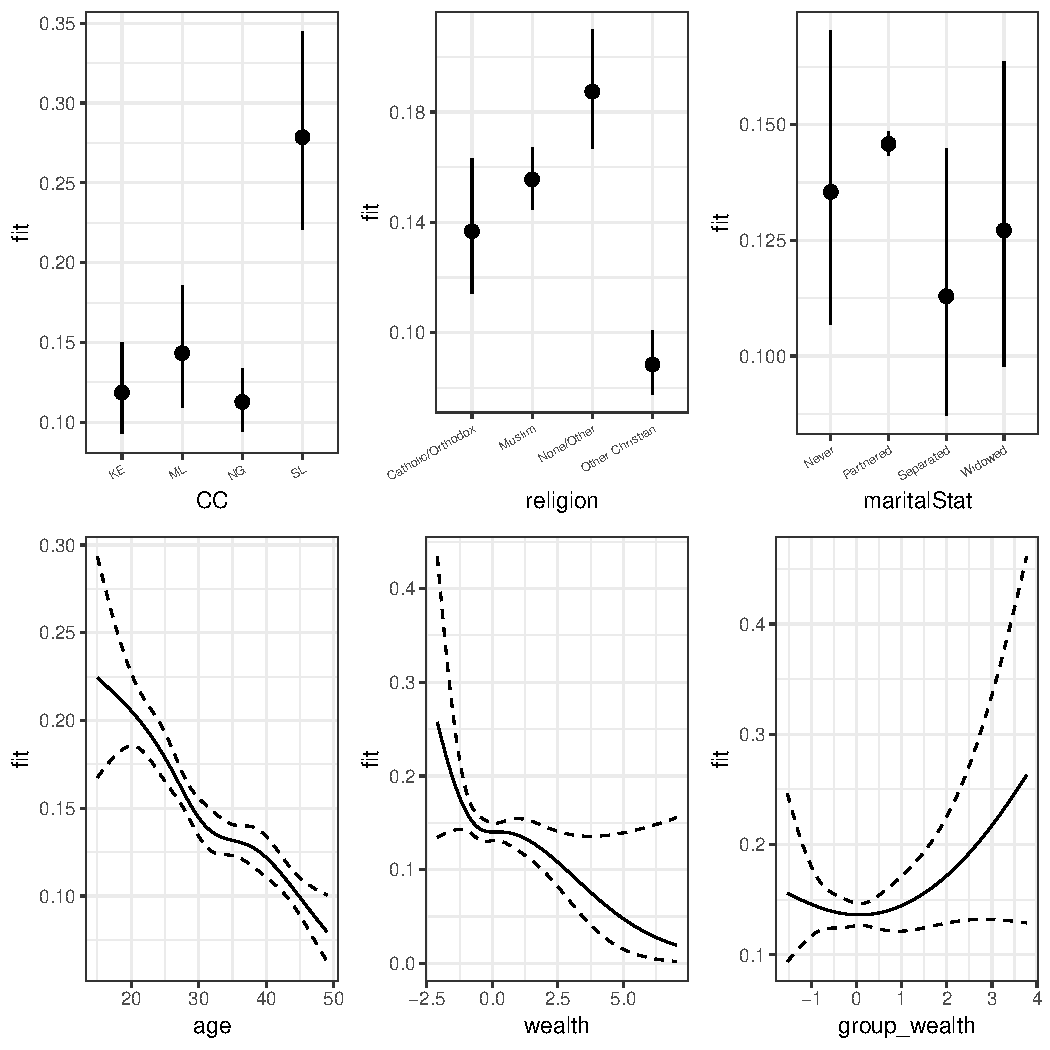
\includegraphics[scale=0.7]{./git_push/daughterPlan_isoplots.Rout.pdf}
\end{figure}
\end{center}

\newpage

\subsection{FGC Persistence}
\begin{center}
\begin{figure}[h!]
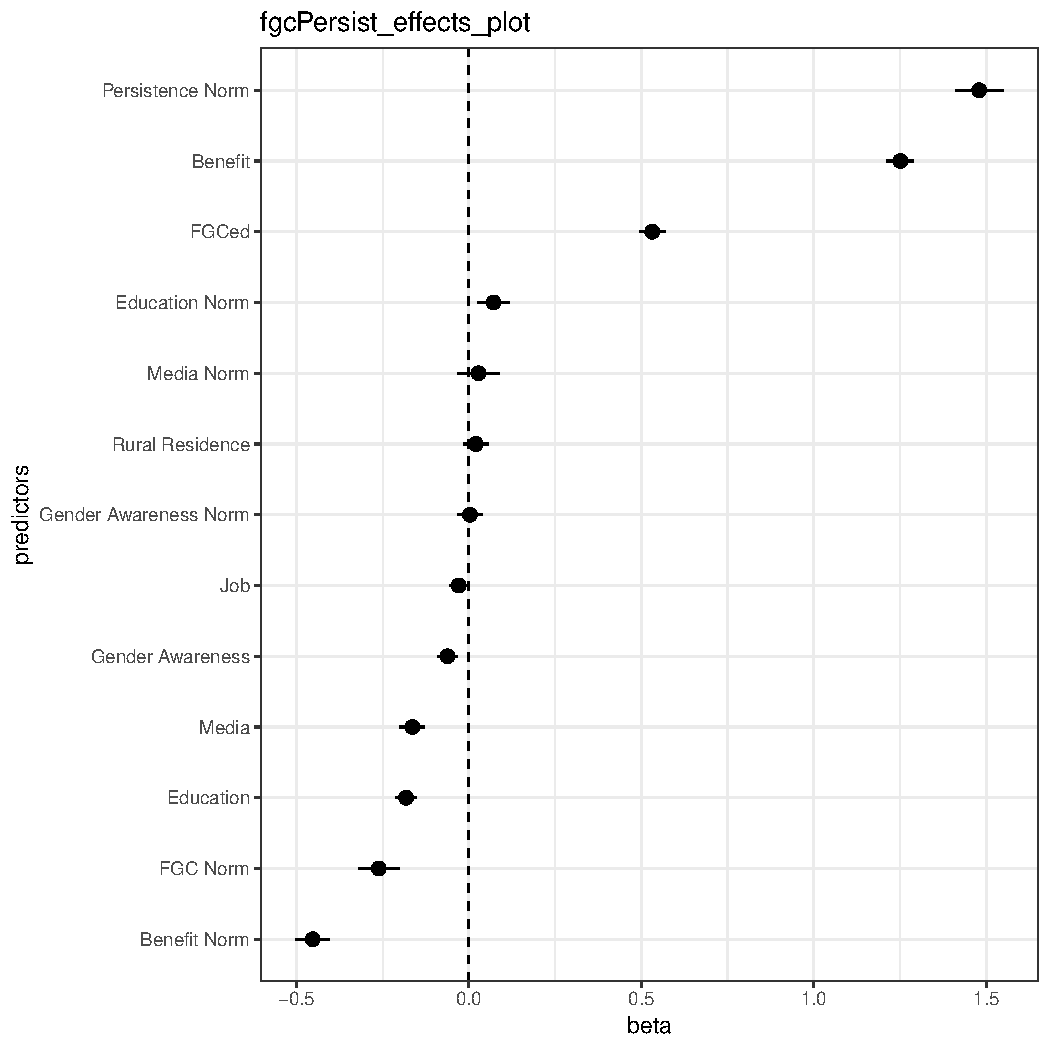
\includegraphics[scale=0.7]{./git_push/fgcPersist_effects_plot.Rout.pdf}
\end{figure}
\end{center}

\begin{center}
\begin{figure}[h!]
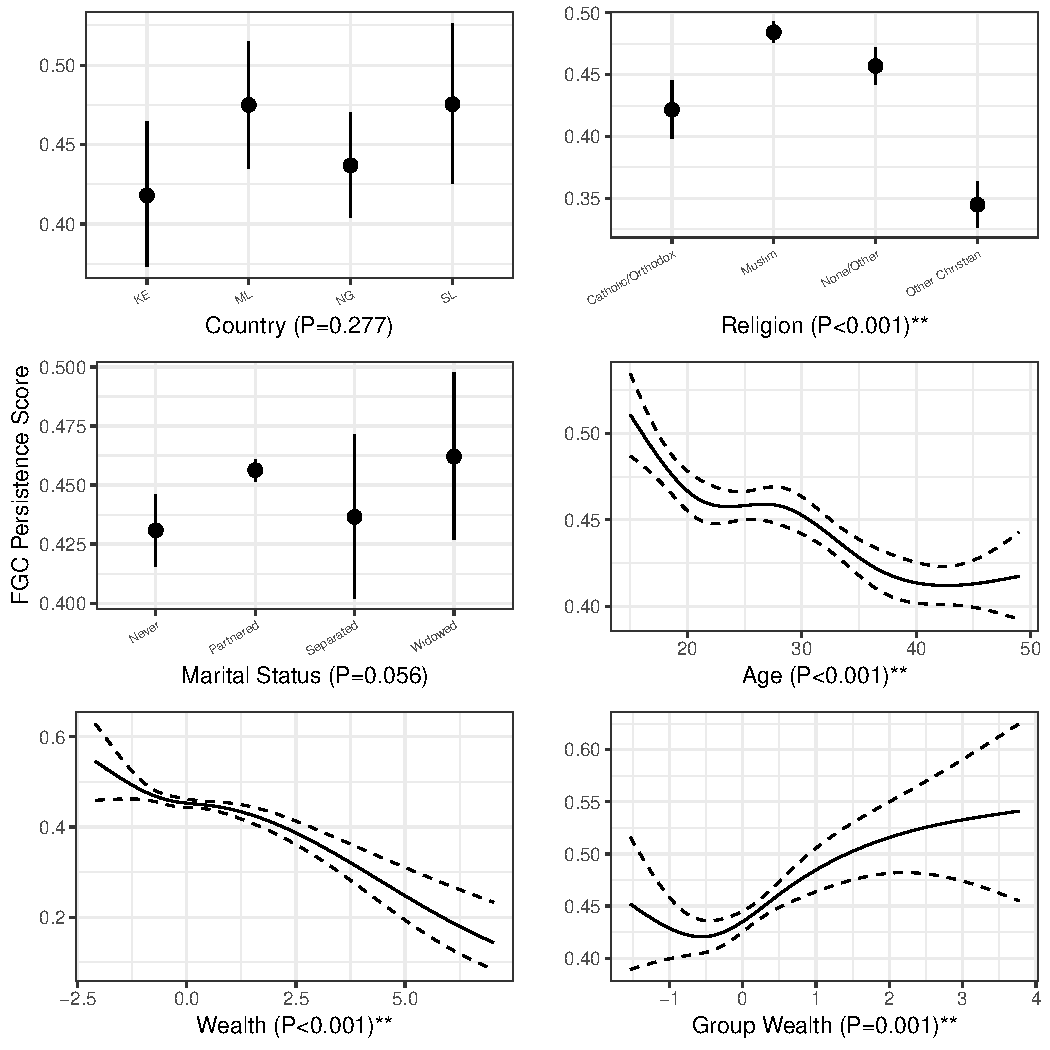
\includegraphics[scale=0.7]{./git_push/fgcPersist_isoplots.Rout.pdf}
\end{figure}
\end{center}

\newpage

\subsection{Hybrid Model}
\begin{center}
\begin{figure}[h!]
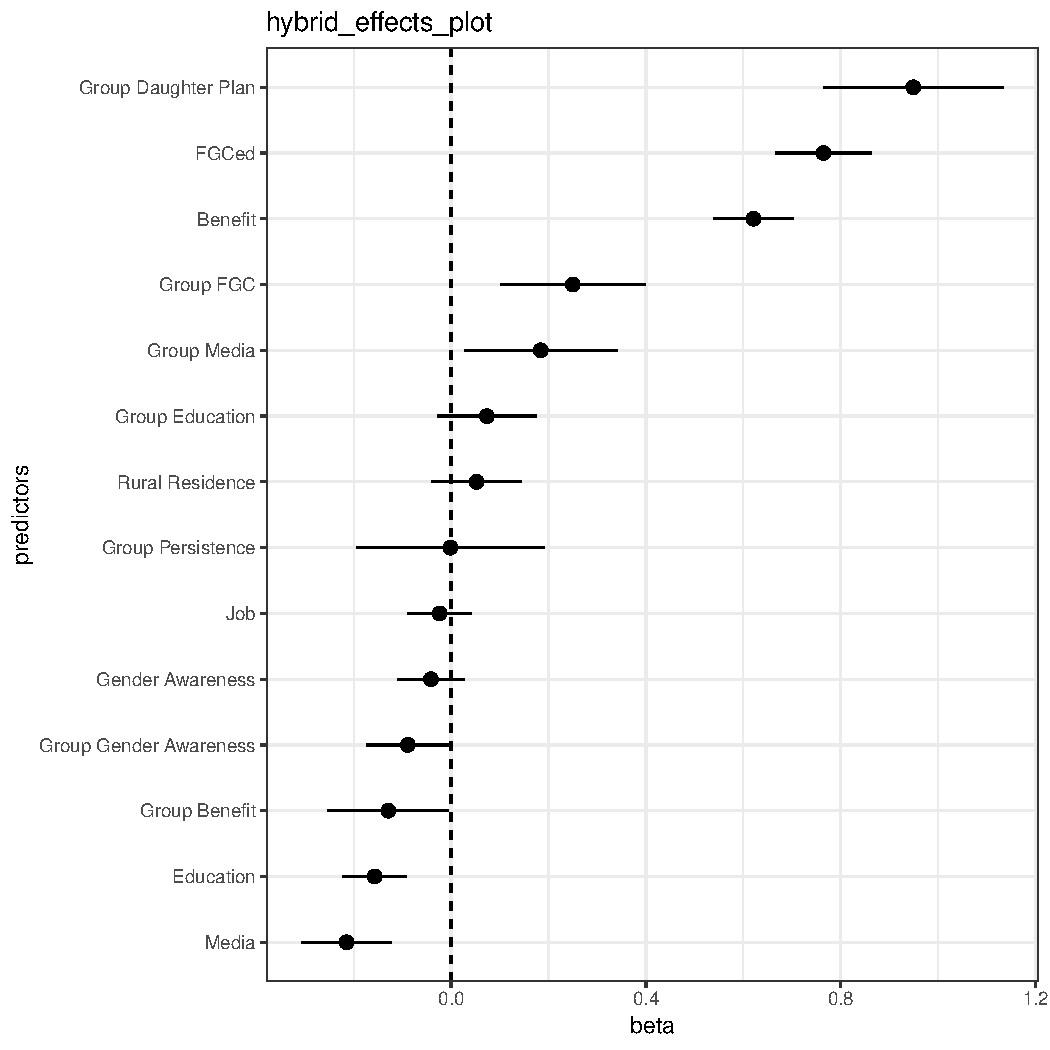
\includegraphics[scale=0.7]{./git_push/hybrid_effects_plot.Rout.pdf}
\end{figure}
\end{center}

\begin{center}
\begin{figure}[h!]
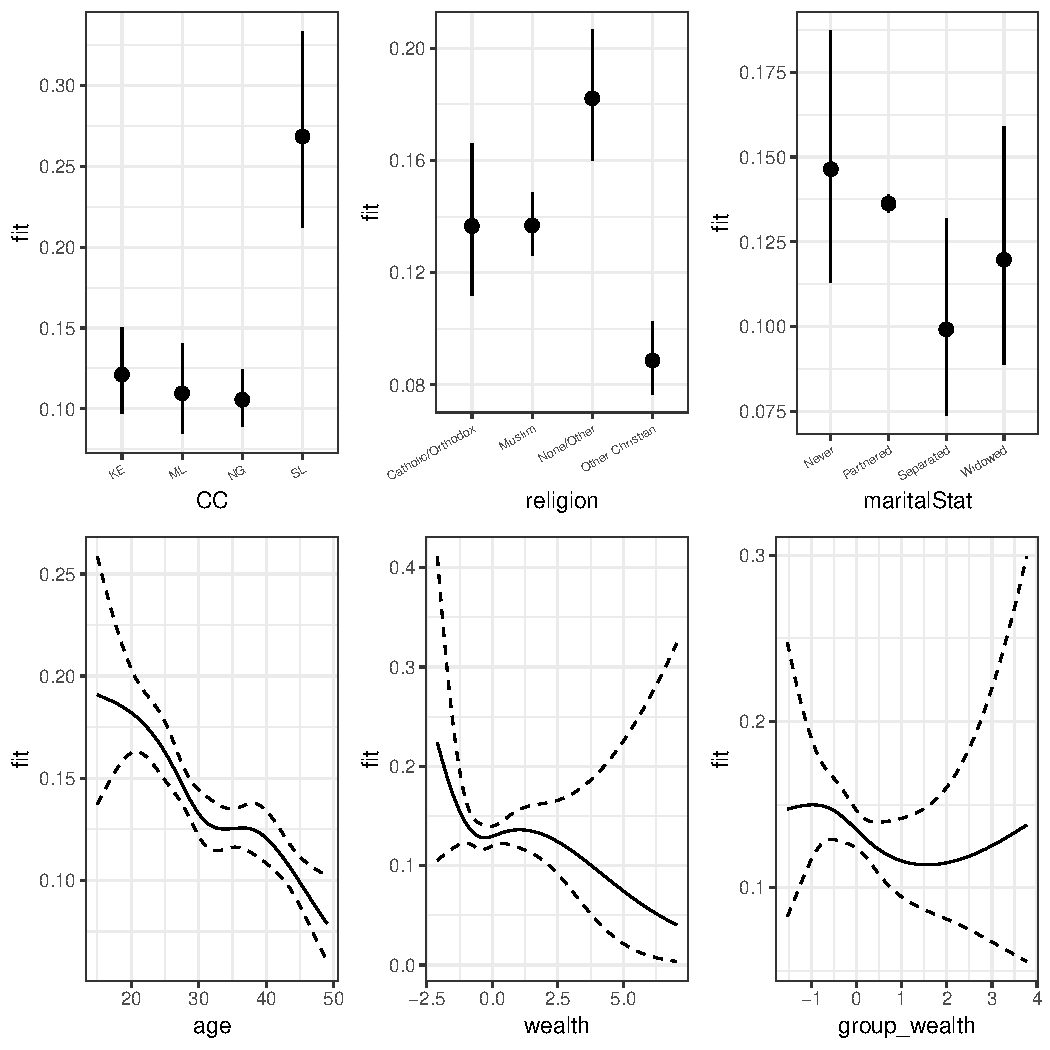
\includegraphics[scale=0.7]{./git_push/hybrid_isoplots.Rout.pdf}
\end{figure}
\end{center}

\begin{center}
\begin{figure}[h!]
\includegraphics[scale=0.7,page=2]{./git_push/hybrid_isoplots.Rout.pdf}
\end{figure}
\end{center}

\FloatBarrier

\bibliography{manual}

\end{document}

